\documentclass{article}

% if you need to pass options to natbib, use, e.g.:
%     \PassOptionsToPackage{numbers, compress}{natbib}
% before loading neurips_2021

% ready for submission
\usepackage[preprint]{neurips_2021}
\usepackage{setspace}
\onehalfspacing

% to compile a preprint version, e.g., for submission to arXiv, add add the
% [preprint] option:
%     \usepackage[preprint]{neurips_2021}

% to compile a camera-ready version, add the [final] option, e.g.:
%     \usepackage[final]{neurips_2021}

% to avoid loading the natbib package, add option nonatbib:
% \usepackage[nonatbib]{neurips_2021}
\usepackage[utf8]{inputenc} % allow utf-8 input
\usepackage[T1]{fontenc}    % use 8-bit T1 fonts
\usepackage[colorlinks = true, 
		    linkcolor = blue,
		    urlcolor  = blue,
            citecolor = blue,
            anchorcolor = blue]{hyperref}       
% hyperlinks
\usepackage{float}
\usepackage{url}            % simple URL typesetting
\usepackage{booktabs}       % professional-quality tables
\usepackage{amsfonts}       % blackboard math symbols
\usepackage{nicefrac}       % compact symbols for 1/2, etc.
\usepackage{microtype}      % microtypography
\usepackage{xcolor}         % colors
\usepackage{natbib}
\usepackage[pdftex]{graphicx}
\usepackage{siunitx} % Required for alignment
\sisetup{
  round-mode          = places, % Rounds numbers
  round-precision     = 2, % to 2 places
}
	
\bibliographystyle{unsrtnat}


\title{Extracting and evaluating concept dependencies from Large Language Models}

% The \author macro works with any number of authors. There are two commands
% used to separate the names and addresses of multiple authors: \And and \AND.
%
% Using \And between authors leaves it to LaTeX to determine where to break the
% lines. Using \AND forces a line break at that point. So, if LaTeX puts 3 of 4
% authors' names on the first line, and the last on the second line, try using
% \AND instead of \And before the third author name.

\author{%
  Dominik Glandorf\\
  Matrikelnummer 6007407\\
  \texttt{dominik.glandorf@student.uni-tuebingen.de} \\
  \And
  Anastasiia Alekseeva\\
  Matrikelnummer 5994775\\
  \texttt{anastasiia.alekseeva@student.uni-tuebingen.de} \\
  \\
  GitHub repository: \url{https://github.com/mlcolab/learning-dependencies}
}

\begin{document}
\vspace*{-5mm}
\maketitle
\vspace*{-5mm}

\begin{abstract}
% What did we do?

% Why did we do it? What did we expect?

% How did we do it?

% What did we find out?

% What now?

\end{abstract}

\section{Introduction}
% Starting broad
% Field of contribution
Large Language Models (LLMs) are trained on immense corpora of text and build on included factual information when performing well in downstream tasks such as question answering. Accessing this knowledge, which is represented by billions of parameters and the network's architecture, has given rise to the research field of Knowledge Extraction from LLMs \citep{cohen2023crawling}, which rests on the assumption that the language models can help retrieve information on the relation between entities. This work contributes to the field and addresses the question of whether LLMs can provide a precise dependency structure of concepts. Apart from the field of knowledge extraction from LLMs, part of computational linguistics, our work contributes to applied education sciences by providing data for computer-assisted education and creating new perspectives for educational knowledge engineering.

% What kind of information do we want to extract?
%% Problem of sequencing in Instructional Design:
Effective and efficient instruction does not only incorporate what to teach but also how to teach it, especially the order of instruction. The empirically proven theory of \textit{Instructional Sequencing} states that prior knowledge of prerequisite learning content or previous exposure to it enhances learning \citep{morrison2019designing}.
% Definition concepts
Within learning contents, \cite{merrill1983component} differentiated facts, concepts, principles, rules, procedures, interpersonal skills, attitudes, and their sole recall from their application.
% TODO: explain this more:
For simplicity, we focus only on concepts such as the "Pythagorean Theorem", which could be a topic for a lecture or a (sub)chapter in a textbook, and do not distinguish between recall and application.
% Concept dependency
% Assumption: information about dependencies between concepts makes instructional sequencing more effective in terms of learning
To be more precise, if one concept is a prerequisite of another, we refer to this relation as a \textit{concept dependency}. For example, to understand the concept of a derivative, knowing the concept of a function will facilitate or even enable learning. Importantly, the dependency relation is distinguished from the similarity, hierarchy, and reference relation \citep{gordon-etal-2016-modeling}. Besides that, the terms prerequisite and concept dependency are used interchangeably. When the concepts are thought of as nodes and the dependencies as directed edges between them, a concept dependency graph emerges, a special type of knowledge graph \citep{wang2016using}. This graph is also called \textit{concept map} in the field of Learning Sciences.
% TODO: provide a (graphical) example of a small concept map
% Why is it important?
The graph can be used to generate ordered reading lists \citep{gordon-etal-2016-modeling}, and hence advance curriculum planning \citep{yang2015concept}, especially for new topics that might not be covered in existing courses. Another use case is automated assessment, where the dependencies can increase the meaning of performance in a task because this can indicate skills in its dependencies \citep{wang2016using}.

% What is our research question?
% How to extract educational concept dependencies that are implicit and evaluate them using existing knowledge sources?
In this work, we tackled the question of how to extract this particular knowledge graph and how to evaluate its quality in a scalable manner.
% What can we contribute/which gap do we sholve?
% 1. No benchmark available -> we set up an evaluation framework based on textbooks and Wikipedia
Our main contributions are the following:
First, there is little research on how to automatically evaluate the precision of extracted concept dependencies, which can be used to train and fine-tune models for this task. Therefore, we propose a set of methods to create baselines for evaluation from two existing unstructured knowledge sources, namely Wikipedia and textbooks. Due to the heuristic character of these methods, we conducted a manual assessment to test their suitability for our purpose. The resulting dataset can be used as a baseline for further research.
% 2. The emerging field of prompt engineering -> we engineered a simple but effective prompt process to query an LLM
Second, the emerging field of prompt engineering provides a constellation of commands to query LLMs, the majority of which are experimental and cannot be considered fully reliable. We propose a method called \textit{output refeeding} that allows mining the educational concept dependencies by sequentially querying the language generation model and transforming its answers into a knowledge graph.

\subsection{Related work}
% Field: Concept Dependency Extraction
% of interest: How are concept dependencies defined?
\cite{talukdar2012crowdsourced} defined the prerequisite relation in terms of the consumption of information about concepts. This coincides with the operationalization of a concept dependency by \cite{gordon-etal-2016-modeling}, who defined it in terms of the helpfulness of learning about another concept and their modeling of information flow to determine the relation. \cite{vuong2011method} defined the relation in terms of performance. More specifically, prior knowledge that leads to a better graduation rate is considered a prerequisite. Concepts are often equated with Wikipedia articles \citep{wang2016prerequisite} but also with results of topic modeling \citep{gordon-etal-2016-modeling}.

% of interest: How are relationships between concepts extracted?
\cite{gordon-etal-2016-modeling} presented two information theoric approaches to extract the dependency relation from a corpus of scientific documents, in which concepts were obtained by a topic model and filtered by human judges. Their entropy-based approach predicts a dependency of concept A on concept B to the extent that the distribution of B can predict the distribution of A. Their information flow approach is also based on co-occurrences of topics in documents but simulates navigation through the documents and considers transitions to documents about other topics as dependencies. Word similarity, citations, and hierarchy served as baselines where word similarity performed better or equally well as the proposed approaches in terms of precision and recall, indicating that their modeled relation is rather symmetric and hence not helpful for sequential curriculum planning.

\cite{liang2015measuring} defined the reference distance metric (RefD) that reflects the extent to which concepts related to concept A (for example by hyperlinks) refer to concepts related to concept B compared to vice versa. If concepts related to A do this more strongly than the other way around, concept A is considered dependent on B. Their proposed measures on Wikipedia concepts performed better than the MaxEntropy classifier on the CrowdComp dataset by \cite{talukdar2012crowdsourced} and their Courses dataset.

More recent approaches already involved neural networks. \cite{gasparetti2022discovering} fed embeddings for the concepts into a number of popular binary classifiers and outperformed the previously referenced methods.  \cite{sun2022conlearn} also worked with concept embeddings but feed them together with a concept dependency graph into a graph neural network to predict the dependency structure between concepts.
% Field: Prompt Engineering for Knowledge Graph creation
% of interest: How can we get internal representations out of a language model?
% Cohen, 2023 
Multiple approaches of prompt engineering for graph creation have been recently developed. Few-shot prompting proved successful \citep{cohen2023crawling}.
% GraphGPT

% Other approaches: Learning Path Analysis and Expert Knowledge
Prerequisites can be also behaviorally inferred from learning paths by testing learners' performance after being presented with different instructional sequences \citep{pavlik2008using,vuong2011method} or analyzing human navigation through information sources \citep{gordon-etal-2016-modeling}. However, these approaches usually lack data, and creating this data has the disadvantage of disengaging users with too difficult concepts before teaching easier or more necessary ones. Experts usually dispose of the required knowledge about concepts to create concept maps. The high cost of expert knowledge motivates the automated extraction of concept dependencies.

\section{Method}
% Section summary
In this section, we will first detail our research design and then the characteristics of our information sources as well as the methods that we used to produce the knowledge graph. 

\subsection{Research design} 
% two baseline methods: textbooks and Wikipedia
% information extraction: one LLM method
% evaluation
% 1. manual inspection via DashBoard
% 2. manual labeling
% 3. convergence between LLM and baselines
The choice of methodology reflects the fact that our research is located at the intersection of education sciences and computational linguistics. On the one hand, we want to achieve a high performance of a state-of-the-art LLM in the downstream task of knowledge graph extraction. On the other hand, we consider a complex educational problem that cannot be purely simplified to classical machine learning metrics but requires additional qualitative assessment to ensure that our results can be educationally sound.

First of all, we restricted the concepts, of which dependencies we assessed, to the domain of linear algebra. This design choice was caused by the assumptions that the highly structured domain of mathematics provides enough relations to capture on the one hand and that linear algebra is a rather mature branch of mathematics where enough data exists for our baselines to be created as well as the LLM to have learned about from its training data. Due to the use of linear algebra in different disciplines, the potential value of results is also increased.

To be able to measure the LLM's performance, we had to come up with a target dataset. This dataset needs to describe a graph, containing the concepts as vertices and their dependencies as directed edges. Since no ground-truth, large-scale knowledge graph of concept dependencies was available to us and might even be impossible to achieve for our educational problem, we chose two sources of educational knowledge to serve as our knowledge base, namely textbooks, and Wikipedia. Due to their end-user-facing format, further processing of the input data (PDFs and webpages) was required to create the above-defined data structure. To make the graphs comparable with each other, the set of concepts was restricted to the union of all concepts indicated in all textbooks' indices. The LLM was prompted and the responses were also further processed to create a knowledge graph.

After creating the baseline datasets and the output to evaluate, we started qualitative evaluation using an interactive dashboard, that visualized the dependency structure. This step was done to get an impression of the general suitability of all three pipelines and identify potential reasons for performance losses. Then a subset of all three datasets was manually rated by multiple raters to not only infer their overall quality but also assess the human performance on the problem. We finally checked for outputs for convergence to give suggestions for a scalable, low-cost evaluation system of future (versions of) LLMs. The former evaluations are rather typical in education research whereas the latter enables the creation of large-scale datasets, potentially suitable to train and fine-tune machine learning models.

\subsection{Baseline extraction}
This section details how we used Wikipedia and textbooks to set up the evaluation baselines for the LLM.

\subsubsection{Wikipedia}
% Why Wikipedia? 
The choice of the online encyclopedia Wikipedia as an educational information source is a result of its inherent graph structure induced by hyperlinks between articles and empirical evidence of its suitability for this purpose \citep{wang2016prerequisite}.
Especially, the platform is claimed to cover concepts up to the complexity of undergraduate curricula to a high extent, which aligns well with our chosen domain of linear algebra, which is usually taught to undergraduate students \citep{yang2015concept}. The focus on dependencies required for understanding a concept makes an encyclopedia an ideal source because its articles are usually written to enable a fast understanding of the article's topic. In an online encyclopedia, hyperlinks provide additional information. In Wikipedia, each content article begins with a summary, often serving as a definition and embedding the topic into its context, before in-depth information follows. In this summary text, we assume an implicit order from most important to least important concepts that are used to explain the topic without digressing to other concepts or unimportant information. The involved concepts are inferred to be a dependency. To prevent direct cycles by two concepts involving each other in their explanation, the one that refers earlier to the other is considered to be dependent on the latter. Situations, where the introduction of concept A states that concept B is dependent on it might be resolved like this.

Our assumptions about the Wikipedia structure were operationalized in the following way to compute the dependencies for a given concept. Every link in the first content paragraph containing a link is considered a candidate dependency. Therefore, any non-content paragraph such as advice regarding irrelevance or missing sources has to be removed beforehand. First, links to categories or fields such as "Mathematics" or "Linear Algebra" are removed based on a manually composed blacklist (a more sophisticated, automatic pruning could make use of Wikipedia's category pages). Then links to articles about persons are filtered out since these do not represent educational concepts. The same applies to links to pages that contain unexpected content such as disambiguation pages. Subsequently, cyclic dependencies are resolved as described above using both character positions of the symmetric links in the text. If more candidates remain than the threshold of 5, only the first 5 were kept, using the assumption of decreasing importance from the beginning on and the constraint of some sparsity of the resulting graph. This set of concepts is then taken as the concept's dependencies. 
%TODO: add the amount of data

The described procedure was executed for every concept in the set resulting from the textbook baseline. Although Wikipedia theoretically offers a larger number of articles about the topic, we decided to stick with the limited set to maintain comparability. However, we decided against restricting the dependencies to concepts in the set to also be able to evaluate the recall of the methods.
% TODO: recall?
The computational complexity of the procedure is relatively low and most time is spent on requesting Wikipedia web pages for the concepts and the links. The overall time was hence reduced by caching the responses to these requests. The technical implementation in Python required engineering our own Wikipedia API using the libraries requests and BeautifulSoap. The tools are used to download the page content and conveniently access elements such as links or special HTML tags indicating that an article is about a person.

\subsubsection{Textbooks}
% Why textbooks?
We chose student textbooks as the complementary information source besides the general purpose knowledge base Wikipedia because they are written by experts specifically for educational knowledge transfer to learners. This does not only lead to comprehensive coverage of carefully selected concepts that are considered relevant by the authors but also to a specific structure that our baseline extraction method exploits, namely a didactic linearization of topics. More precisely, the authors are expected to first introduce concepts that later introduced concepts build upon. Another useful structure in textbooks is the index, which provides a comprehensive list of concepts defined as its entities and covered in the book, and indicates the area of introduction.

% Amount of data
Due to the popularity of the topic of Linear Algebra, we could easily identify ten free textbooks on the topic and obtain their PDF representations (either directly typeset in this format or scanned and processed with optical character recognition). The books comprised 584 pages on average (652,297 characters) and disposed of a median of 382 index entries.

% Steps of processing
% preprocessing

% Wikisearch: query Wikipedia search engine for keyword (and field) and rank results based on Levenshtein distance
First, the textbooks were converted from PDF to unformatted text. To identify all concepts of interest covered in a book, the pages containing the index were identified and each index entry with its corresponding pages was extracted in a semi-manual fashion. This required setting parameters such as the title, position of the text columns, and the types of nesting and delimiters. To enable comparing the knowledge graph across the baselines, we decided to use the set of Wikipedia articles as the set of possible concepts, meaning that only a Wikipedia article title can serve as a vertex in the knowledge graph. This required to map from each index entry to the closest Wikipedia article. For this disambiguation, the index entry was introduced into the Wikipedia search engine suffixed with the field term "(Mathematics)" to hint at the general area. Due to the high diversity of the resulting ten articles, their titles were string-matched with the search term (excluding the suffix) using the Levenshtein distance (provided by a Python library). The article title with the lowest Levenshtein distance that did not refer to a disambiguation page was the result of this so-called \textit{Wikisearch disambiguation}.

% relation extraction

% entity recognition and disambiguation
For dependency extraction, we came up with two distinct strategies.
% order pruning:  identify unlikely dependencies based on a certain number of books that introduce concepts in a particular order
The first is solely based on indices whereas the latter also uses the full text. The first strategy is called \textit{order pruning} and is focused on unlikely dependencies on the graph. It checks whether two concepts are introduced at least twice in a specific order and rules out the dependency that is not suggested by this order. For example, if concept A is introduced twice before concept B, it is unlikely to depend on a concept introduced later by two independent authors. To create a sparse graph, this strategy requires a massive amount of books, which was not available to us, but it can help to prune dependencies and refine a candidate graph.

% common introductory usage: identify other concepts that are most often mentioned on the first page given in the index across all books
This candidate graph is the output of the second heuristic called \textit{common introductory usage}. This is based on a similar rationale as the Wikipedia heuristic because it figures out which other concepts are used to introduce a new concept. The first and rather structured source of information is the index, again. Some books list multiple pages for index entries, indicating that the concept occurs again at a later point in a significant way. If concept A appears for the second time on the first page for concept B, A is likely to be a dependency of B. However, the structured source of index entries has a low amount of data, which led to the involvement of the full text. Here, entity recognition plays a crucial role because not every word is a concept of interest and not every concept occurs with its canonical title in natural text.

% Wikifier: identify entity mentions using link targets and PageRank
One convenient method is provided by the Wikifier \citep{brank2017annotating}. The underlying algorithm looks for links in the entire Wikipedia with the link text matching a word in the input. Naturally, the same text can link to distinct articles, which requires disambiguation based on the context. Wikifier solves this by creating a graph based on all potential links and uses a PageRank algorithm to calculate the score for each potential link target. We restricted links to correspond to a link text of at least 3 characters to get rid of abbreviations that were contained in formulas randomly. We used a minimum PageRank of 0.00005 as a threshold after manual inspection aimed at a good recall of links but also good precision. The Wikifier was called via its online API. All detected link targets on the first page of an index entry serve as candidate dependencies which are then ranked by the following three criteria: First, the number of books in which it occurs in the area of introduction. Second, the average number of occurrences in these books. Third, the PageRank of the link. As with the Wikipedia dependencies, only the 5 highest-ranking candidates are saved as dependencies in the knowledge graph. This procedure was carried out for all index entries across all books.

The final resulting graph is the union of dependencies identified by the two common introductory usage sources (indices and full text), pruned by the unlikely dependencies from order pruning.

\subsection{LLM extraction}
% description of T0PP and our infrastructure
% • Fine-tuned BLOOM on several question-answering datasets
% • 11 billion parameters () • ~3-10 seconds per request on our infrastructure
Due to the closed-source character of the very powerful and successful language model GPT3 by openai and the unavailability of an API for its most recent application ChatGPT, we decided to use the open-source model BLOOM by bigscience, which is a joint effort by hundreds of researchers around the world and is based on the same transformers architecture as GPT3 and has a comparable amount of parameters. Because of resource limitations and our specific use case, we used a derived model called \textit{T0pp} (https://huggingface.co/bigscience/T0pp), which only has 11 billion parameters and is fine-tuned for zero-shot task generalization, especially question-answering. The dataset used for training T0pp is also available under the name P3 (Public Pool of Prompts) (https://huggingface.co/datasets/bigscience/P3). We set up the language model on the cloud infrastructure of the university's excellence cluster and ran it in generation mode (no training) with a maximum response length of 50 tokens on a node with eight cores of the type Nvidia GeForce RTX 2080 Ti. This model consumed approximately 44GB of RAM and a typical request took three to ten seconds to be answered completely. To save time loading the model into the memory, we set up an HTTP server to conveniently query the model via GET requests from our local machines.

% description of the extraction procedure
% 1. output refeeding
% first prompt: {definition} := What is the mathematical definition of {concept}?
% second prompt:  {list of dependencies} := What mathematics concepts are mentioned here: {definition}
% 2. response parsing to Wikipedia article
% {canonical list of dependencies} :=Wikisearch disambiguation on {list of dependencies}
Manual inspection of our chosen and other LLMs' responses (such as meta's Galactica) has led to the following procedure to extract dependencies from the knowledge base of T0pp, which we call \textit{output refeeding}. It is based on the previously explained assumption that understanding a concept requires understanding other concepts involved in its definition. Given a concept of interest, we therefore first prompt the model for a definition of the concept: "What is the mathematical definition of {concept}?" The response is defined as {definition} and involved in the second prompt: "What mathematical concepts are mentioned here: {definition}". The model usually responds with a comma-separated list that is split by commas and then disambiguated in the same way as the index entries in the textbook baseline by our Wikisearch disambiguation. Finally, self-dependencies, that might occur during this procedure, are deleted from the set of dependencies. This procedure is run for the same set of concepts as the Wikipedia baseline.

\begin{figure}
    \centering
    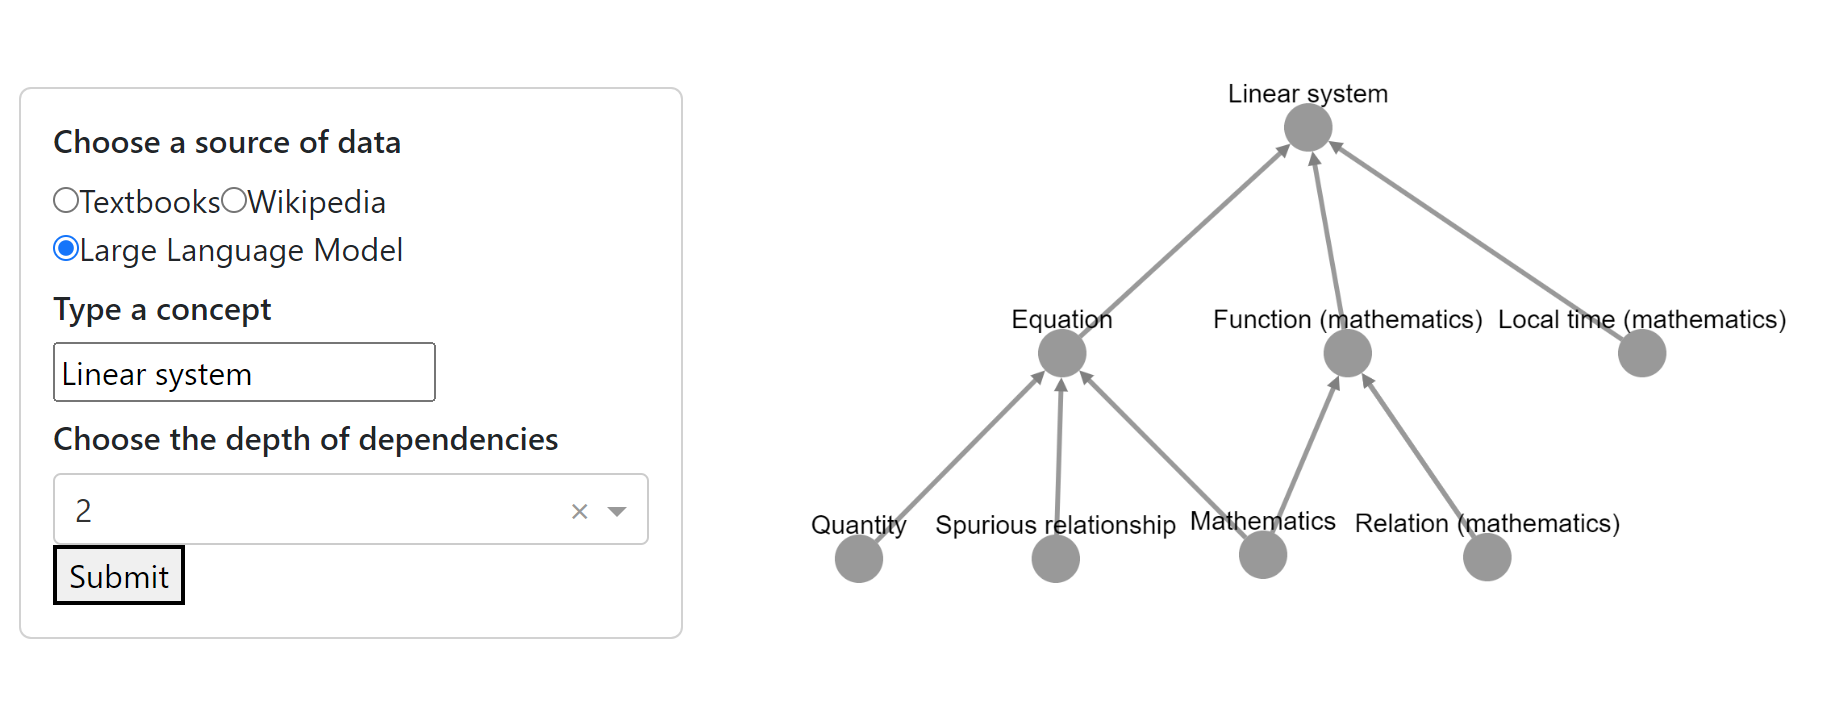
\includegraphics[width=.95\textwidth]{img/dash_example.png}
    \caption{A screenshot of the interactive application.}
    \label{fig:dash_example}
\end{figure}

\subsection{Manual inspection via Dashboard}
As indicated in our design, this educational problem requires also a qualitative evaluation. We hence developed a Dashboard via graphing library for Python Plotly\footnote{https://plotly.com/python/} (Fig.\ref{fig:dash_example}). The application is devised so that one could examine the resulting graph itself in a convenient environment. It allows plotting the concept dependencies graphs for three knowledge sources and types of dependency mining methods (LLM, Wikipedia, and textbooks) for different depths of dependencies, meaning that dependencies of dependencies are shown. The dashboard also has potential use for educators that are interested in concept dependencies.

\subsection{Manual baseline}
% procedure to assess the accuracy of the output
The novel character of our baselines and the resulting uncertainty about their appropriateness to evaluate the LLM's performance motivated us to evaluate all three knowledge graphs independently before checking their convergence. Therefore, 4 raters were presented with 100 dependencies from each graph and had to rate them in a binary fashion (correct vs incorrect). We only evaluated the quality of dependencies for concepts that occurred at least in 50\% of the textbooks to ensure that there is enough data for the textbook baseline and that we assess the data for important concepts only. For the ratings, we calculated Cohen's Kappa as a measure of interrater reliability. This should not only guarantee the confidence of the performance evaluation but also assess the difficulty of the problems for human raters.

\subsection{Baseline consistency}
% for which concepts did we compare what to see what
Consistency of the LLM with the baselines is the most scalable measure because the baselines can be created automatically and hence be used to evaluate large numbers of LLM outputs or even fine-tune the model for this specific downstream task. First-order consistency is fulfilled for a concept dependency extracted from the LLM if it is a direct dependency for this concept also in the baseline. Second-order consistency is fulfilled if a dependency is among the direct dependencies or the dependencies of dependencies in the baseline. We are interested in the relative number of consistent dependencies between the LLM and the baseline because this gives an estimate of the precision of the predictions. However, it is also helpful to measure the recall by calculating the relative number of baseline dependencies that were correctly guessed. In the first-order consistency, this is just a change in the denominator. 

\section{Results}
% Case Study using Dashboard

%Manual baseline
% Interrater reliability
% How good are the baselines?
% How good is the LLM?
% diagram


\begin{figure}[H]
    \centering
    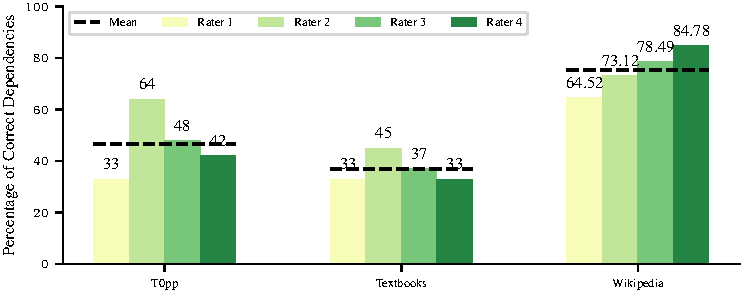
\includegraphics[width=.95\textwidth]{img/rating.pdf}
    \caption{Rating.}
    \label{fig:rating}
\end{figure}

\begin{figure}[H]
    \centering
    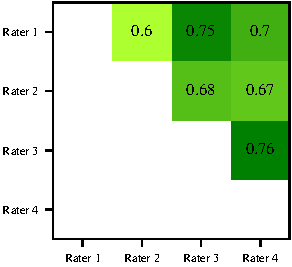
\includegraphics[width=.4\textwidth]{img/kappa.pdf}
    \caption{Interrater reliability, kappa coefficient.}
    \label{fig:kappa}
\end{figure}

%Convergence statistics
% diagram for similarity of outputs

\begin{figure}
    \centering
    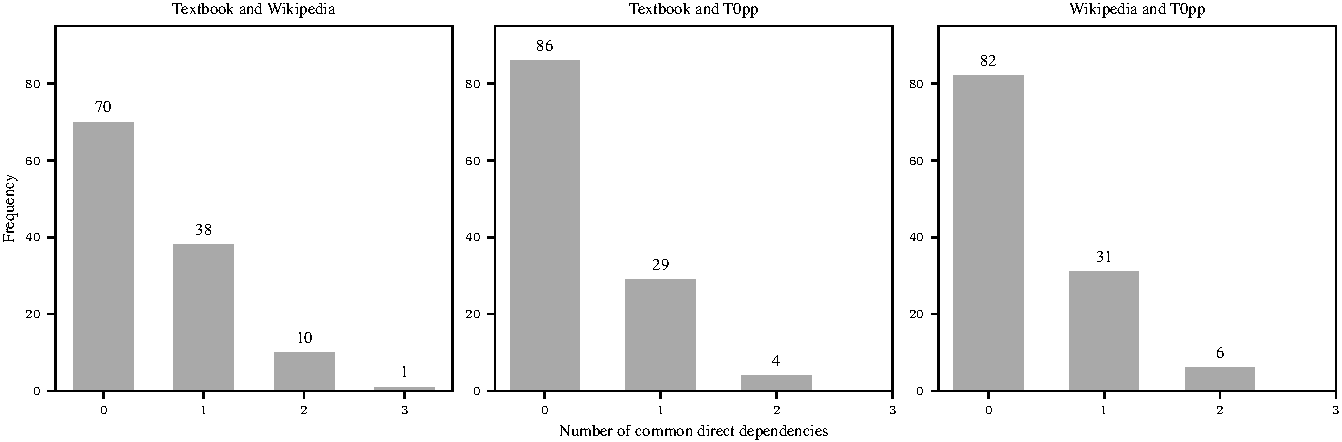
\includegraphics[width=.95\textwidth]{img/comp_direct_deps.pdf}
    \caption{Convergence metrics. Number of common direct dependencies between sources.}
    \label{fig:comp_direct_deps}
\end{figure}

\section{Discussion}
% What is our main result?
% we can make the implicit knowledge explicit far above chance level
% problem is very complex -> humans do not fully agree
% Wikipedia might be the best source to automatically evaluate the output

% What are potential flaws?

% disambiguation already includes noise
% error propagation


% we only evaluated up to two levels of the graph, not the graph as a whole. different levels of abstractions in extracted dependencies
% (in)direct cycles
% is there even something like a gold standard? some educational reflection about different didactic approaches and more depth than just understanding the definition of a topic
% Cohen et al (2023) think that there is no gold standard or ground truth.

Each information extraction method is not fully independent of the other, in particular, entity recognition and concept disambiguation steps in the procedure for LLM and textbooks depend on Wikipedia.

% we are still using the language generator, so it is just another downstream task, maybe it is more of a philosophical question what is implicit/explicit knowledge


% + "I don't know" option in the prompt engineering part
% + Google search

% Q: Outlook and Future research ideas:

As shown, current LLMs are not sufficiently precise in creating concept maps, which confirms previous research \cite{hwang2021comet}. This could be improved by training the pre-trained models on the knowledge graph data mined from Wikipedia or any other reliable sources of concept dependencies in a specific subject of instruction \cite{west2022symbolic}.
% advancements in LLMs that are interesting for us
% use cases in education

\section{Acknowledgements}
We sincerely thank our project supervisors, Álvaro Tejero-Cantero and Hanqi Zhou.

\bibliography{references.bib}

\newpage


\section{Appendix}



\begin{figure}[H]
    \centering
    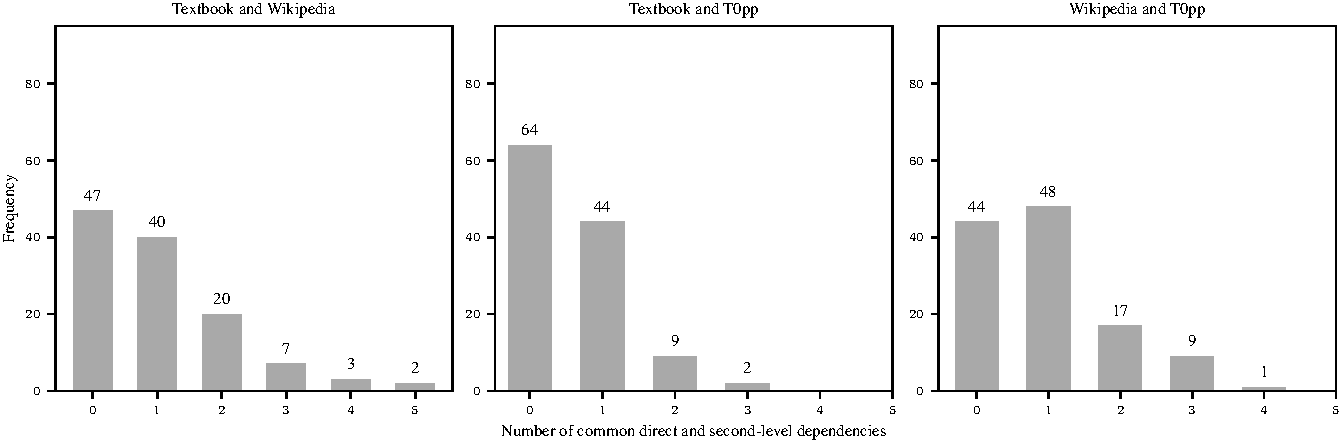
\includegraphics[width=.95\textwidth]{img/comp_second_deps.pdf}
    \caption{Convergence metrics. Number of common direct and second-level dependencies between sources.}
    \label{fig:comp_second_deps}
\end{figure}






\end{document}
